In this chapter, you will learn how to make
free-standing wheat sourdough bread.

\begin{figure}[!htb]
  \includegraphics[width=\textwidth]{loaf-pan-free-standing.jpg}
  \caption{A free-standing sourdough bread made with wheat flour}
\end{figure}

A free-standing sourdough bread is my favorite
type of bread. It combines a great crunchy crust, superb
flavor, and a soft fluffy crumb. This is the type of bread
that is being inhaled by my friends and family. Unfortunately
making this type of bread requires a lot more effort, patience,
and technique than other types of bread. You have to perfectly
balance the fermentation process. You can not ferment for too
short and also not for too long. The techniques you need to
learn require a bit more skill. It took me several attempts
to get this right. One of the challenges I faced was that
I had the wrong flour. I didn't properly know how to use my oven.
When should I stop the fermentation? There is a lot of information
out there. I dug through most of it and have tried almost everything.
In many cases the information was wrong, in other cases, I
found another valuable puzzle piece. Aggregating all this
information was one of my main motivations to start the bread code.
My key learning was that there there is no recipe that
you can blindly follow. You will always have to adapt the recipe
to your local available tools and environment.

But do not worry. After reading this chapter you will know
all the signs to look out for. You will be able to read your dough.
You will turn into a confident hobby baker that can bake bread
at home, at high altitudes, at low altitudes, in summer, in winter,
at your friend's place, and even on vacation. Furthermore,
you will know how to scale your production from 1 bread to 100 loaves of bread.
If you ever wanted to open up a bakery, consider this knowledge to
be your foundation.

Mastering this process will enable you to bake amazing bread without
ever buying yeast again.

\section{The process}

\begin{figure}[!htb]
  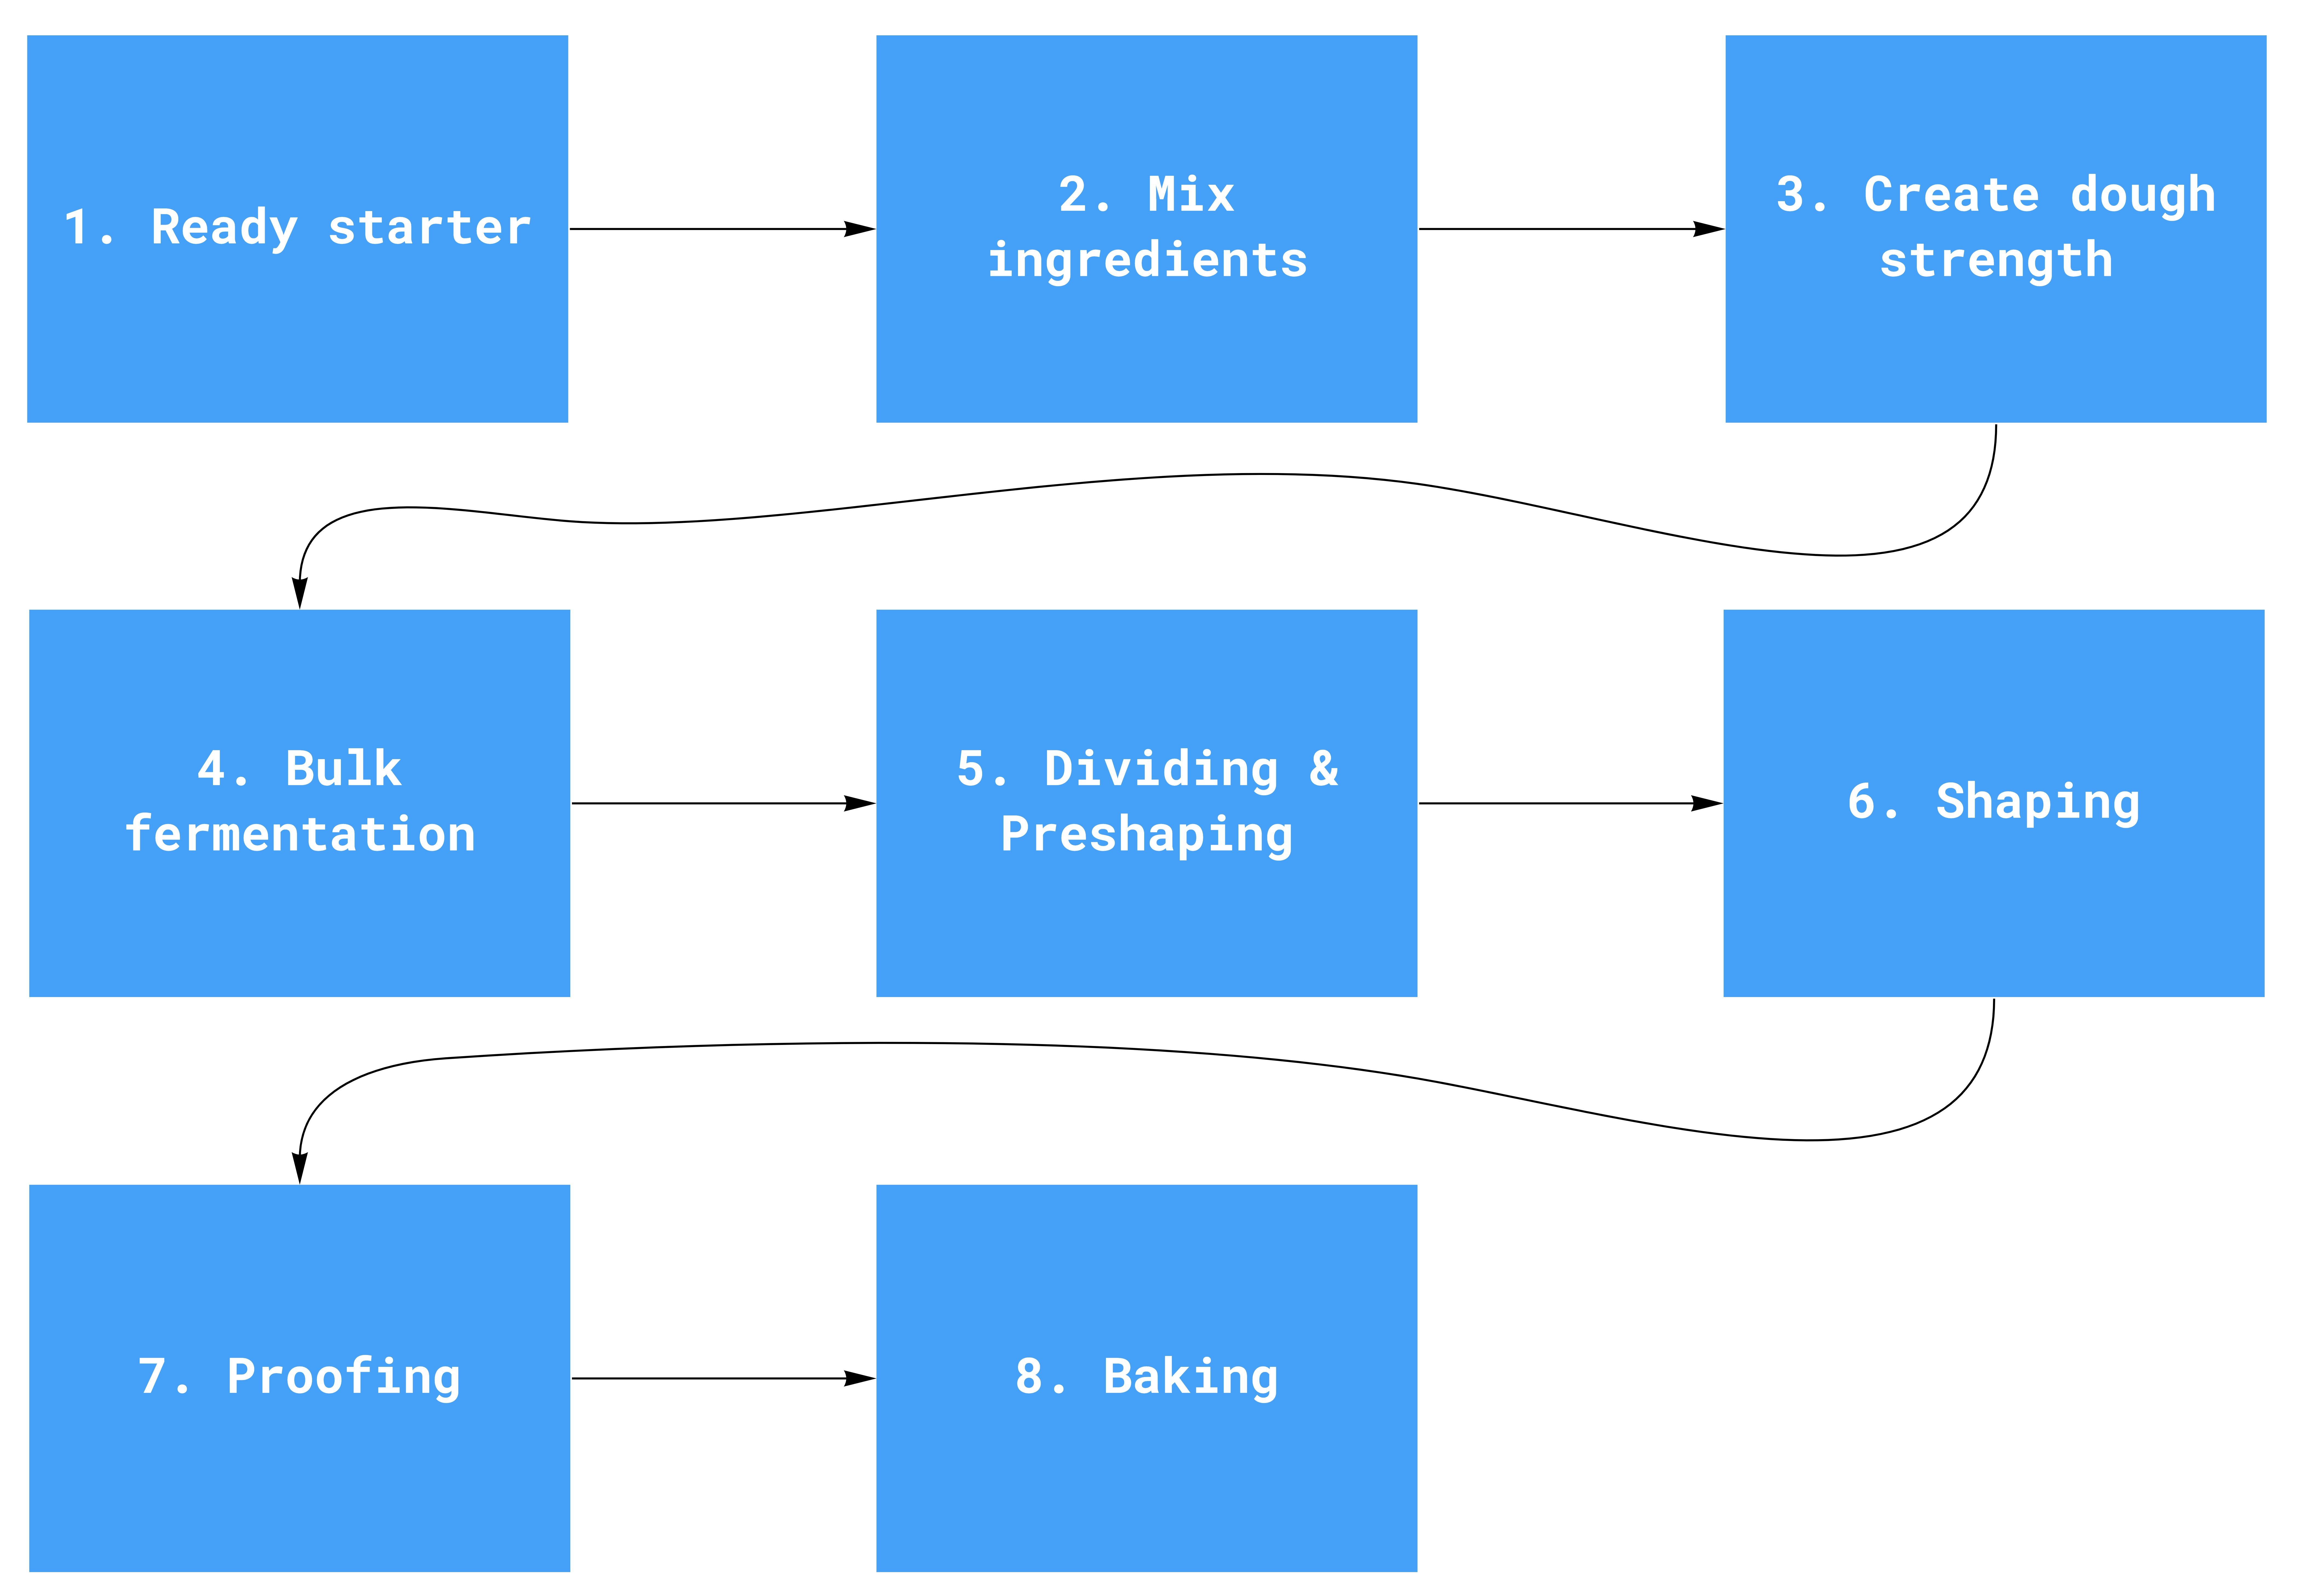
\includegraphics[width=\textwidth]{sourdough-process-overview.jpg}
  \caption{An overview of the whole sourdough process from start to finish}
\end{figure}

The whole process of making great sourdough bread starts with
readying your sourdough starter. The key to mastering
this process is to manage the fermentation process properly.
For this, the basis is to have an active and healthy
sourdough starter.

Once your starter is ready you proceed to mix all the ingredients.
You want to homogenize your sourdough starter properly. This
way you ensure an even fermentation across your whole dough.

After a short break, you will proceed and create dough strength.
Kneading will create a strong gluten network. This is essential
to properly trap the CO2 created during the fermentation.

Once you kneaded the bulk fermentation starts. Bulk fermentation
because you typically ferment multiple doughs together in one bulk.
Understanding when to stop this step will take some practice.
But nothing to worry about, you will learn the exact signs to look out for.

Once this is completed you need to divide your large blob of
dough into smaller pieces and preshape each piece. This allows
you to apply more dough strength and shape more uniform loaves.

The proofing stage follows where you finish the fermentation process.
Depending on your time you can proof at room temperature or in the fridge.
Mastering proofing will turn your good loaf into a great loaf.

Lastly, you will finish the whole process by baking. You will learn different
options on how to properly steam your dough. This way your
dough will have a beautiful oven spring. During the second
stage of the baking process, you will finish building your crust.

All the steps rely on each other. You will need to get each of
the steps right to make the perfect bread.

\section{Readying your starter}

The most crucial part of the bread-making process is your starter.
The starter is what starts the fermentation in your main dough.
If your starter is off, then your main dough is also going
to cause trouble during the fermentation. Your starter's
properties are passed on to your main dough. If your starter
doesn't have a good balance of yeast to bacteria, so will your
main dough.

\begin{figure}[!p]
  \centering
  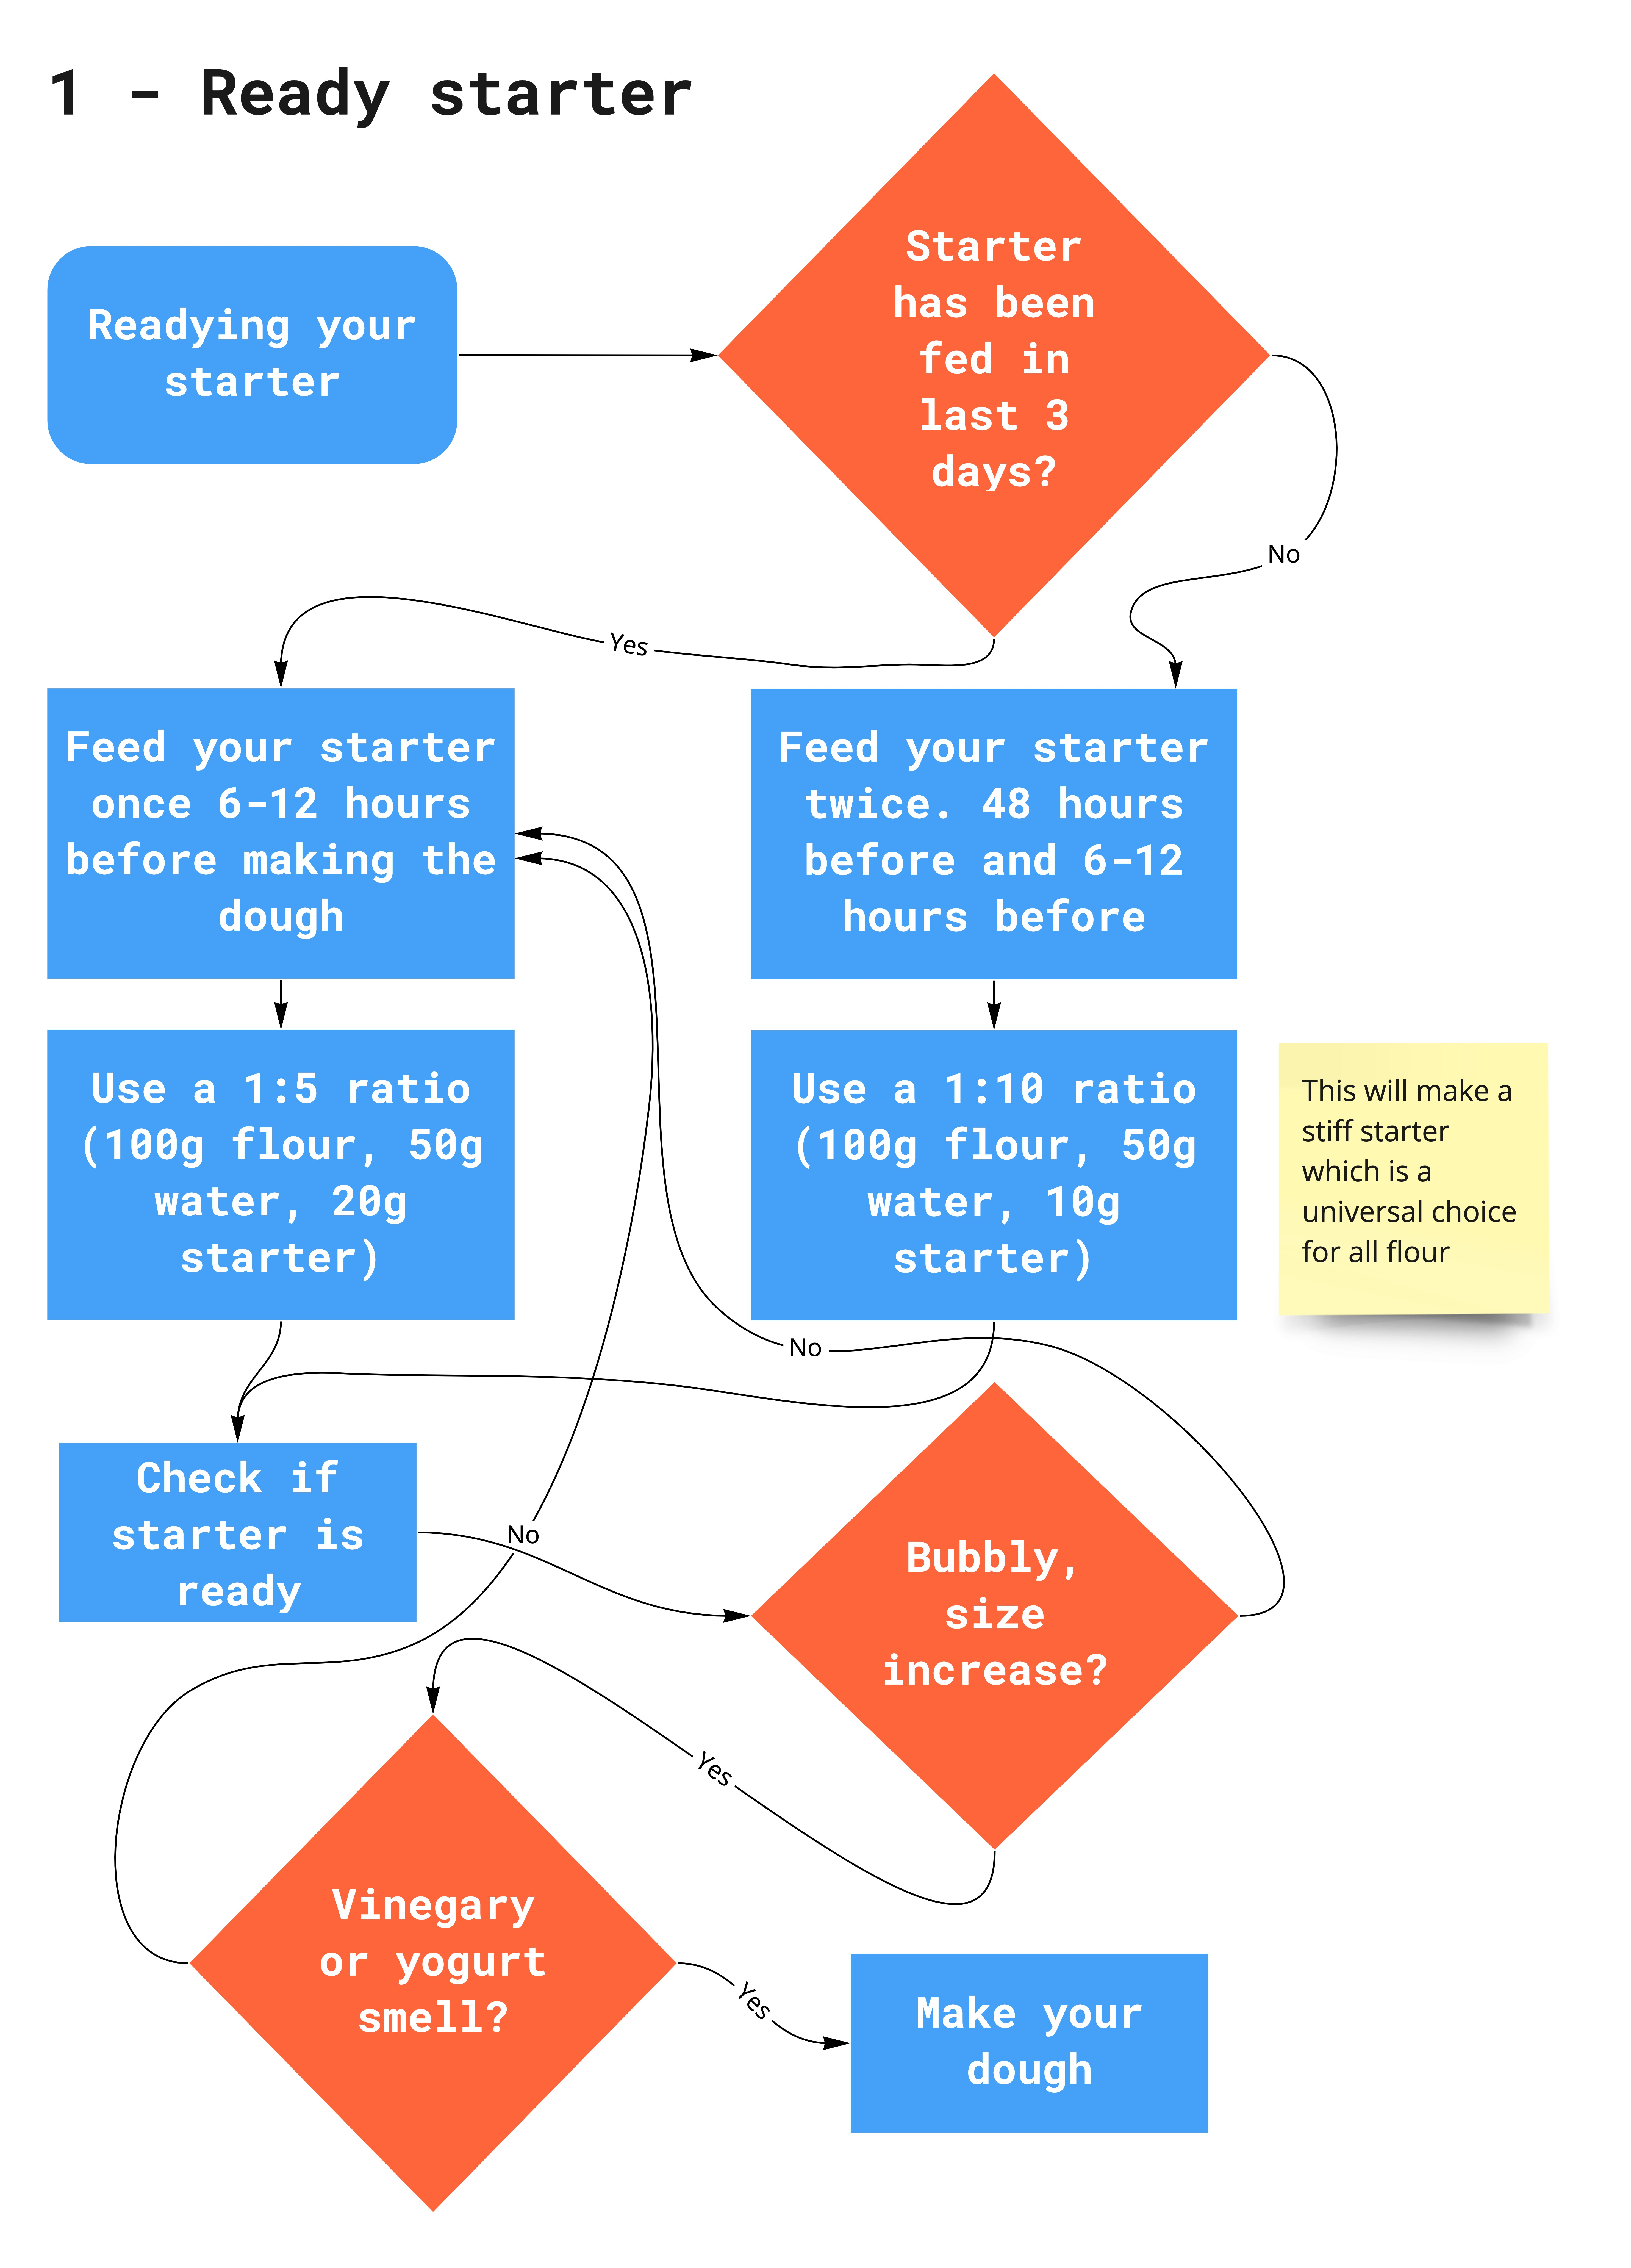
\includegraphics[width=\textwidth]{1-ready-starter}
  \caption[Readying a starter]{A flowchart showing how you can prepare your starter before baking.
  This assumes you are using a stiff starter.}
\end{figure}

Generally, think of the dough you are mixing as a big starter with salt.
After mixing all the ingredients you have a green field environment again.
The yeast and bacteria start to fight again to outcompete each other.
There is plenty of food available and they all do their best to win.
Depending on the starter you mix into your dough some of the microorganisms
might have an advantage over the others.

The first option to achieve a good balance is to apply feedings.
If your starter hasn't been fed in a long period the
bacteria dominate. This happens if your starter has been
sitting unused in the fridge for instance. As more and more
acidity piles up the environment is becoming more and more hostile
to the yeast. The lactic acid bacteria tolerate this environment
better. Your dough fermentation would be more towards the
bacterial side with this starter. By applying a couple of
feedings the yeast becomes more active. The older your
starter the more acid resistant the yeast becomes. Initially,
I had to feed my starter 2-3 times to fix the balance. With my
more mature starter, one feeding seems to be enough to balance
the microorganisms.

Some people use a 1:1:1 ratio to refresh the starter. This would
be one part of the old starter (10g for instance), 1 part of flour,
and one part of water. I think this is utter rubbish. As mentioned
your starter is a gigantic dough. You would never a 1:1:1 ratio to
make a dough. You might use a maximum of 20 percent starter to
make a dough. That's why I advocate using a 1:5:5 ratio or a
1:10:10 ratio depending on how ripe your starter is. As I almost
always use a stiffer sourdough starter due to its enhanced
yeast fermentation advantages (see section \ref{section:stiff-starter})
my ratio is never 1:5:5. My ratio would be 1:5:2.5 (1 part old starter,
5 parts flour, 2.5 parts water). If it is very warm where you live
you could opt for the aforementioned 1:10:5 or 1:20:10. This
way you slow down the ripening of your starter. You can use this
trick too to make starter feeding work with your schedule.
If your starter is typically ready in 6 hours but today you need it
ready later, simply increase how much flour/water you feed your starter.
These are all values that you need to experiment with on your own.
Every starter is unique and might behave slightly differently.

The second option at your disposal is the starter quantity that
you use to make the dough. As previously stated your starter
regrows inside of your main dough. While I would normally use
10-20 percent of starter based on the flour, sometimes I go
as low as 1 percent starter. This way the microorganisms have
more room to balance out while fermenting the dough. If my sourdough
starter has not been fed in a day I might use 5 percent of sourdough
to make a dough.  If I push this to 2 days without feedings
I lower the starter amount even further. I would opt for the
previously mentioned 1 percent starter. If the food is very scarce
your microorganisms will sporulate. They need to regrow again
from the spores they created. In this hibernation state, it takes
longer for them to become fully active again. I have tried
several times to make dough directly out of a dry starter.
I wasn't successful because the fermentation took too long.
The microorganisms had to regrow from spores and then begin
the fermentation. As explained earlier there is a limit to
fermentation times as your dough naturally breaks down.
Furthermore, you want your microorganisms to outcompete
other pathogens contained in the flour. The less starter
you use the easier it is for them to reproduce. A strong
starter will outcompete other germs. While the method of
reducing the starter works, I recommend option one more.
It will reliably create better bread. Option 2 is typically
what I use when I fed my starter in the morning but didn't
manage to make a dough in the evening. I don't want to feed
my starter again the next morning. I would like to make a dough
directly without waiting and thus use less of the very ripe starter.

Over time you will become more accustomed to your starter
and how it behaves. You will be able to read the signs of its
activity and judge its state.



\section{Ingredients}

This chapter is still pending and will be added soon.

\section{Hydration}
This chapter is still pending and will be added soon.

\section{Autolyse}
This chapter is still pending and will be added soon.

\section{Fermentolyse}
This chapter is still pending and will be added soon.

\section{Dough strength}
This chapter is still pending and will be added soon.

\section{Controlling fermentation}
This chapter is still pending and will be added soon.

\section{Optional Preshaping}
This chapter is still pending and will be added soon.

\section{Shaping}
This chapter is still pending and will be added soon.

\section{Proofing}
This chapter is still pending and will be added soon.

\section{Scoring}
This chapter is still pending and will be added soon.
